% alfak2 sparse joint model: the two-time-point fit, whose steps every path shares.
% Mirrors fit_sparse_joint(), sparse_joint_problem(), sparse_joint_domain(),
% sparse_joint_optimise_scales(), sparse_joint_posterior() and
% predict.alfak2_sparse_joint_fit() in R/. Build: pdflatex flow_core.tex
\documentclass[tikz,border=4pt]{standalone}
% Shared style of the alfak2 flowcharts (doc/flowcharts/*.tex).
% Each chart is a standalone document; build one with
%   cd doc/flowcharts && pdflatex <chart>.tex
% or all of them with doc/flowcharts/build.sh. doc/alfak2_method.tex includes
% the PDFs.
\usepackage{amsmath,amssymb}
\usepackage[scaled=0.92]{helvet}
\renewcommand{\familydefault}{\sfdefault}
\usepackage{xcolor}
\usetikzlibrary{positioning,shapes.geometric,shapes.misc,arrows.meta,calc,fit,backgrounds}

% Thresholds of series = "auto" (sparse_joint_auto_thresholds in
% R/sparse-joint-series-methods.R). Change them here when the code changes.
\newcommand{\autoshare}{0.3}
\newcommand{\autoweight}{0.5}

\newcommand{\code}[1]{\texttt{\small #1}}

\definecolor{cIn}{HTML}{DCE6F2}    \definecolor{cInB}{HTML}{4F6D9A}
\definecolor{cProc}{HTML}{F5F5F5}  \definecolor{cProcB}{HTML}{707070}
\definecolor{cDec}{HTML}{FFF2CC}   \definecolor{cDecB}{HTML}{B8902B}
\definecolor{cTwo}{HTML}{D0E4F5}   \definecolor{cTwoB}{HTML}{2E6DA4}
\definecolor{cAnch}{HTML}{D9EAD3}  \definecolor{cAnchB}{HTML}{3D7A33}
\definecolor{cPair}{HTML}{FCE5CD}  \definecolor{cPairB}{HTML}{C0661A}
\definecolor{cState}{HTML}{E6DDF2} \definecolor{cStateB}{HTML}{6A4A9C}
\definecolor{cCore}{HTML}{EFEFEF}  \definecolor{cCoreB}{HTML}{8A8A8A}
\definecolor{cOut}{HTML}{D5EDEA}   \definecolor{cOutB}{HTML}{2C7C73}
\definecolor{cErr}{HTML}{F8D7D7}   \definecolor{cErrB}{HTML}{B03030}
\definecolor{cAuto}{HTML}{FFFBEA}

\tikzset{
  >={Stealth[length=2.4mm,width=1.8mm]},
  every node/.style={font=\small},
  box/.style={draw=#1B, fill=#1, rounded corners=2.5pt, line width=0.7pt, align=left,
              inner xsep=5pt, inner ysep=4pt},
  box/.default=cProc,
  w/.style={text width=#1},
  dec/.style={draw=cDecB, fill=cDec, chamfered rectangle, chamfered rectangle xsep=7pt,
              line width=0.7pt, align=center, inner xsep=3pt, inner ysep=3pt},
  err/.style={box=cErr, font=\footnotesize},
  tag/.style={draw=#1, dashed, rounded corners=6pt, fill=white, font=\scriptsize, inner sep=2.5pt,
              align=center},
  arr/.style={->, line width=0.8pt, draw=black!75},
  darr/.style={->, line width=0.8pt, draw=black!60, dashed},
  lab/.style={font=\footnotesize\itshape, fill=white, inner sep=1.5pt, text=black!85},
  frame/.style={draw=#1, rounded corners=6pt, line width=0.9pt, inner sep=7pt},
  ftitle/.style={font=\footnotesize\bfseries, fill=white, inner sep=2pt, text=#1},
}

\begin{document}
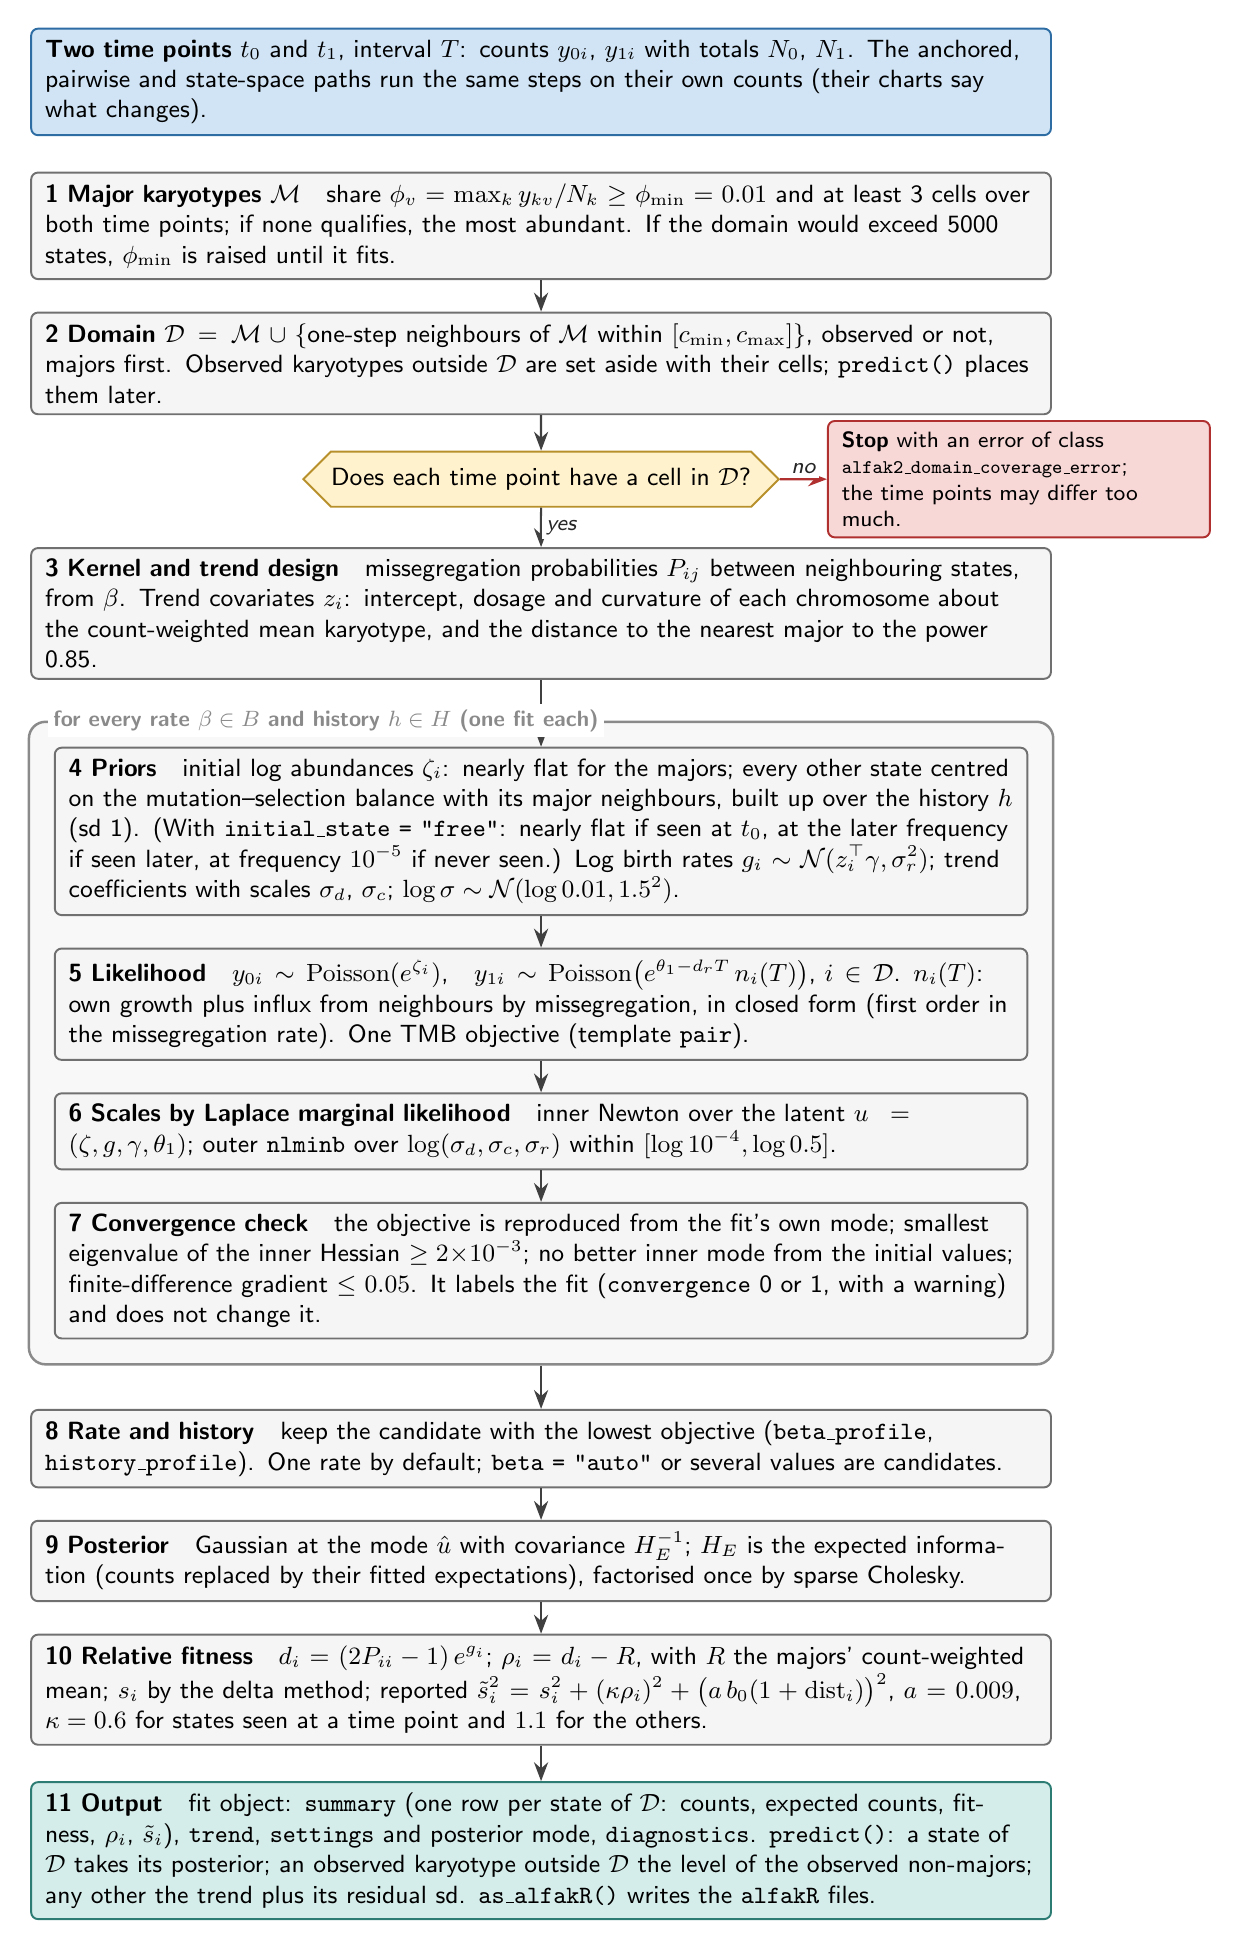
\begin{tikzpicture}

\node[box=cTwo, w=12.6cm] (in) at (0,0) {%
  \textbf{Two time points} $t_0$ and $t_1$, interval $T$: counts $y_{0i}$, $y_{1i}$ with totals $N_0$, $N_1$.
  The anchored, pairwise and state-space paths run the same steps on their own counts (their charts say
  what changes).};

\node[box, w=12.6cm, below=0.45cm of in] (major) {%
  \textbf{1 Major karyotypes $\mathcal M$}\quad share $\phi_v=\max_k y_{kv}/N_k\ge\phi_{\min}=0.01$ and at
  least 3 cells over both time points; if none qualifies, the most abundant. If the domain would
  exceed 5000 states, $\phi_{\min}$ is raised until it fits.};
\node[box, w=12.6cm, below=0.4cm of major] (domain) {%
  \textbf{2 Domain} $\mathcal D=\mathcal M\cup\{$one-step neighbours of $\mathcal M$ within
  $[c_{\min},c_{\max}]\}$, observed or not, majors first. Observed karyotypes outside $\mathcal D$ are
  set aside with their cells; \code{predict()} places them later.};
\node[dec, below=0.45cm of domain] (cover) {Does each time point have a cell in $\mathcal D$?};
\node[err, w=4.5cm, right=0.6cm of cover] (stop) {%
  \textbf{Stop} with an error of class\\ {\ttfamily\scriptsize alfak2\_domain\_coverage\_error};\\ the time points may differ too much.};
\draw[arr] (major) -- (domain);
\draw[arr] (domain) -- (cover);
\draw[arr, draw=cErrB] (cover) -- node[lab, above] {no} (stop);

\node[box, w=12.6cm, below=0.5cm of cover] (kernel) {%
  \textbf{3 Kernel and trend design}\quad missegregation probabilities $P_{ij}$ between neighbouring
  states, from $\beta$. Trend covariates $z_i$: intercept, dosage and curvature of each chromosome about
  the count-weighted mean karyotype, and the distance to the nearest major to the power 0.85.};
\draw[arr] (cover) -- node[lab, right] {yes} (kernel);

\node[box, w=12.0cm, below=0.85cm of kernel] (prior) {%
  \textbf{4 Priors}\quad initial log abundances $\zeta_i$: nearly flat for the majors; every other
  state centred on the mutation--selection balance with its major neighbours, built up over the history
  $h$ (sd 1). (With \code{initial\_state = "free"}: nearly flat if seen at $t_0$, at the later frequency
  if seen later, at frequency $10^{-5}$ if never seen.) Log birth rates
  $g_i\sim\mathcal N(z_i^\top\gamma,\sigma_r^2)$; trend coefficients with scales $\sigma_d$, $\sigma_c$;
  $\log\sigma\sim\mathcal N(\log0.01,1.5^2)$.};
\node[box, w=12.0cm, below=0.4cm of prior] (lik) {%
  \textbf{5 Likelihood}\quad $y_{0i}\sim\mathrm{Poisson}(e^{\zeta_i})$,\quad
  $y_{1i}\sim\mathrm{Poisson}\bigl(e^{\theta_1-d_rT}\,n_i(T)\bigr)$, $i\in\mathcal D$.
  $n_i(T)$: own growth plus influx from neighbours by missegregation, in closed form (first order in the
  missegregation rate). One TMB objective (template \code{pair}).};
\node[box, w=12.0cm, below=0.4cm of lik] (laplace) {%
  \textbf{6 Scales by Laplace marginal likelihood}\quad inner Newton over the latent
  $u=(\zeta,g,\gamma,\theta_1)$; outer \code{nlminb} over $\log(\sigma_d,\sigma_c,\sigma_r)$ within
  $[\log10^{-4},\log0.5]$.};
\node[box, w=12.0cm, below=0.4cm of laplace] (check) {%
  \textbf{7 Convergence check}\quad the objective is reproduced from the fit's own mode; smallest
  eigenvalue of the inner Hessian $\ge2\times10^{-3}$; no better inner mode from the initial values;
  finite-difference gradient $\le0.05$. It labels the fit (\code{convergence} 0 or 1, with a warning)
  and does not change it.};
\draw[arr] (kernel) -- (prior);
\draw[arr] (prior) -- (lik);
\draw[arr] (lik) -- (laplace);
\draw[arr] (laplace) -- (check);
\begin{scope}[on background layer]
  \node[frame=cCoreB, fill=cCore!45, fit=(prior)(lik)(laplace)(check), inner xsep=9pt, inner ysep=9pt] (loop) {};
\end{scope}
\node[ftitle=cCoreB, anchor=west, fill=white] at ($(loop.north west)+(0.25,0)$)
  {for every rate $\beta\in B$ and history $h\in H$ (one fit each)};

\node[box, w=12.6cm, below=0.55cm of loop] (best) {%
  \textbf{8 Rate and history}\quad keep the candidate with the lowest objective (\code{beta\_profile},
  \code{history\_profile}). One rate by default; \code{beta = "auto"} or several values are candidates.};
\node[box, w=12.6cm, below=0.4cm of best] (post) {%
  \textbf{9 Posterior}\quad Gaussian at the mode $\hat u$ with covariance $H_E^{-1}$; $H_E$ is the
  expected information (counts replaced by their fitted expectations), factorised once by sparse
  Cholesky.};
\node[box, w=12.6cm, below=0.4cm of post] (rel) {%
  \textbf{10 Relative fitness}\quad $d_i=(2P_{ii}-1)\,e^{g_i}$; $\rho_i=d_i-R$, with $R$ the majors'
  count-weighted mean; $s_i$ by the delta method; reported
  $\tilde s_i^2=s_i^2+(\kappa\rho_i)^2+\bigl(a\,b_0(1+\mathrm{dist}_i)\bigr)^2$, $a=0.009$,
  $\kappa=0.6$ for states seen at a time point and $1.1$ for the others.};
\draw[arr] (loop) -- (best);
\draw[arr] (best) -- (post);
\draw[arr] (post) -- (rel);

\node[box=cOut, w=12.6cm, below=0.45cm of rel] (out) {%
  \textbf{11 Output}\quad fit object: \code{summary} (one row per state of $\mathcal D$: counts, expected
  counts, fitness, $\rho_i$, $\tilde s_i$), \code{trend}, \code{settings} and posterior mode,
  \code{diagnostics}. \code{predict()}: a state of $\mathcal D$ takes its posterior; an observed
  karyotype outside $\mathcal D$ the level of the observed non-majors; any other the trend plus its
  residual sd. \code{as\_alfakR()} writes the \code{alfakR} files.};
\draw[arr] (rel) -- (out);

\end{tikzpicture}
\end{document}
